\documentclass[hyperref={pdfpagelabels=false},table,10pt]{beamer}     %mathserif,


%%%%%%%%%%%%%%%%%%%%%%%%%%%%%% BEGIN-Packages %%%%%%%%%%%%%%%%%%%%%%%%%%%%%
\usepackage{amsmath,amssymb,amsfonts}
\usepackage{mathrsfs,enumerate}
\usepackage{color,xcolor}
\usepackage{graphicx,subfigure}
\usepackage{clock} % Use this package to insert a clock in the beamer.
\usepackage{textcomp}
\usepackage[T1]{fontenc}
\usepackage{verbatim}
\usepackage{moreverb}
\usepackage{booktabs}
\usepackage{tabularx}
\usepackage{multirow,multicol}
\usepackage{natbib}
\usepackage[ruled,lined,linesnumbered]{algorithm2e}
%\usepackage{algorithm2e}
%\usepackage{url}
%\usepackage{hyperref}
\usepackage[colorlinks,linkcolor=black,citecolor=black,urlcolor=black]{hyperref}%[colorlinks,linkcolor=blue,citecolor=blue,urlcolor=blue]
\usepackage{CJK}
%%%%%%%%%%%%%%%%%%%%%%%%%%%%%%%% END-Packages %%%%%%%%%%%%%%%%%%%%%%%%%%%%%


% \setbeamertemplate{navigation symbols}{} % Disable the buttons at the bottom.

\graphicspath{{Figures/}} % Set the directory where figures are saved.

%%%%%%%%%%%%%%%%%%%% BEGIN-Theorem-like Environments %%%%%%%%%%%%%%%%%%%%%
%\newtheorem{mybox}{}
\newtheorem{Con}{Conjecture}[section]
\newtheorem{Thm}{Theorem}[section]
\newtheorem{Prop}{Proposition}[Thm]
%%%%%%%%%%%%%%%%%%%%% END-Theorem-like Environments %%%%%%%%%%%%%%%%%%%%%%


%%%%%%%%%%%%%%%%%%%%%%%%%% BEGIN-New Commands %%%%%%%%%%%%%%%%%%%%%%%%%%%%
\newcommand{\email}[1]{\href{mailto: #1}{\tt {\color{blue}#1}}}
\newcommand{\red}{\color{red}}
\newcommand{\blue}{\color{blue}}
\newcommand{\green}{\color{green}}
\newcommand{\brown}{\color{brown}}
\newcommand{\orange}{\color{orange}}
\newcommand{\yellow}{\color{yellow}}
\newcommand{\white}{\color{white}}
\newcommand{\Real}{\mathbb{R}}
\newcommand{\Tran}[1]{#1^\mathrm{T}}
\newcommand{\st}{\textnormal{s.t.}}
\newcommand{\dist}{\textnormal{dist}}
\newcommand{\bc}{\begin{center}}
\newcommand{\ec}{\end{center}}
\newcommand{\bl}{\begin{flushleft}}
\newcommand{\el}{\end{flushleft}}
\newcommand{\tbf}{\textbf}
\newcommand{\be}{\begin{equation}}
\newcommand{\ee}{\end{equation}}
\newcommand{\ba}{\begin{array}}
\newcommand{\ea}{\end{array}}
\newcommand{\btab}{\begin{table}\begin{tabular}}
\newcommand{\etab}{\end{tabular}\end{table}}
\newcommand{\nn}{\nonumber}
\newcommand{\xn}{x_1,x_2,\ldots,x_n}
\newcommand{\framee}[2]{\frame{\frametitle{#1} #2}}
\newcommand{\reff}[1]{(\ref{#1})} % 免得敲()
\newcommand{\inner}[2]{\left\langle#1,#2\right\rangle}
\newcommand{\paper}[1]{({\blue \footnotesize{#1}})}
\newcommand{\hd}[1]{\multicolumn{1}{c}{#1}}


\newcommand{\rmnum}[1]{\romannumeral #1}
\newcommand{\Rmnum}[1]{\expandafter\@slowromancap\romannumeral #1@}
%%%%%%%%%%%%%%%%%%%%%%%%%%%% END-New Commands %%%%%%%%%%%%%%%%%%%%%%%%%%%%

\usepackage[lined,linesnumbered,rightnl,ruled]{algorithm2e}

\begin{document}
\begin{CJK*}{GBK}{kai}

\title[distance geometry]{\textsc{A Buildup-based Error Minimization Method with Application to Protein Structure Determination}}
\author[Zhenli Sheng]{Zhenli Sheng (ʢ����)\\email: {\blue szl@lsec.cc.ac.cn}}
% \institute{Institute of Computational Mathematics and Scientific/Engineering Computing}
\institute[ICMSEC, CAS]{Institute of Computational Mathematics and Scientific/Engineering Computing,\\Chinese Academy of Sciences}
\date[]{April 9th, 2013\\ seminar talk}
\frame{
\titlepage
}

% File Name: ThankYou.tex
% Function: Insert an Outline page.


\section*{\textsc{Outline}}
\begin{frame}
\frametitle{\textsc{Outline}}
\end{frame}

\begin{frame}
\frametitle{\textsc{Outline}}
\tableofcontents[pausesections]
\end{frame}

\section{Problem introduction}
\frame{
\frametitle{Distance Geometry Problem}
Find the coordinate vectors $x_{1},x_{2},\ldots,x_{n}$ that satisfy several given distances between them. Mathematically, this problem can be stated as follow, \\
\vspace{0.5cm}
\red{
Find $x_{1},x_{2},\ldots,x_{n}$, such that
\begin{displaymath}
\|x_{i}-x_{j}\|=d_{i,j},\quad (i,j) \in S.
\end{displaymath}
or
\begin{displaymath}
l_{i,j}\leq \|x_{i}-x_{j}\|\leq u_{i,j},\quad (i,j) \in S.
\end{displaymath}
}
\begin{itemize}
  \item The data given may have some errors.
  \item This problem can be formulated as global optimization problem.
  \item It has many applications.
\end{itemize}
}

\frame{
\frametitle{Application \Rmnum{1}: Graph Realization}
\begin{figure}
  \centering
  \subfigure{ 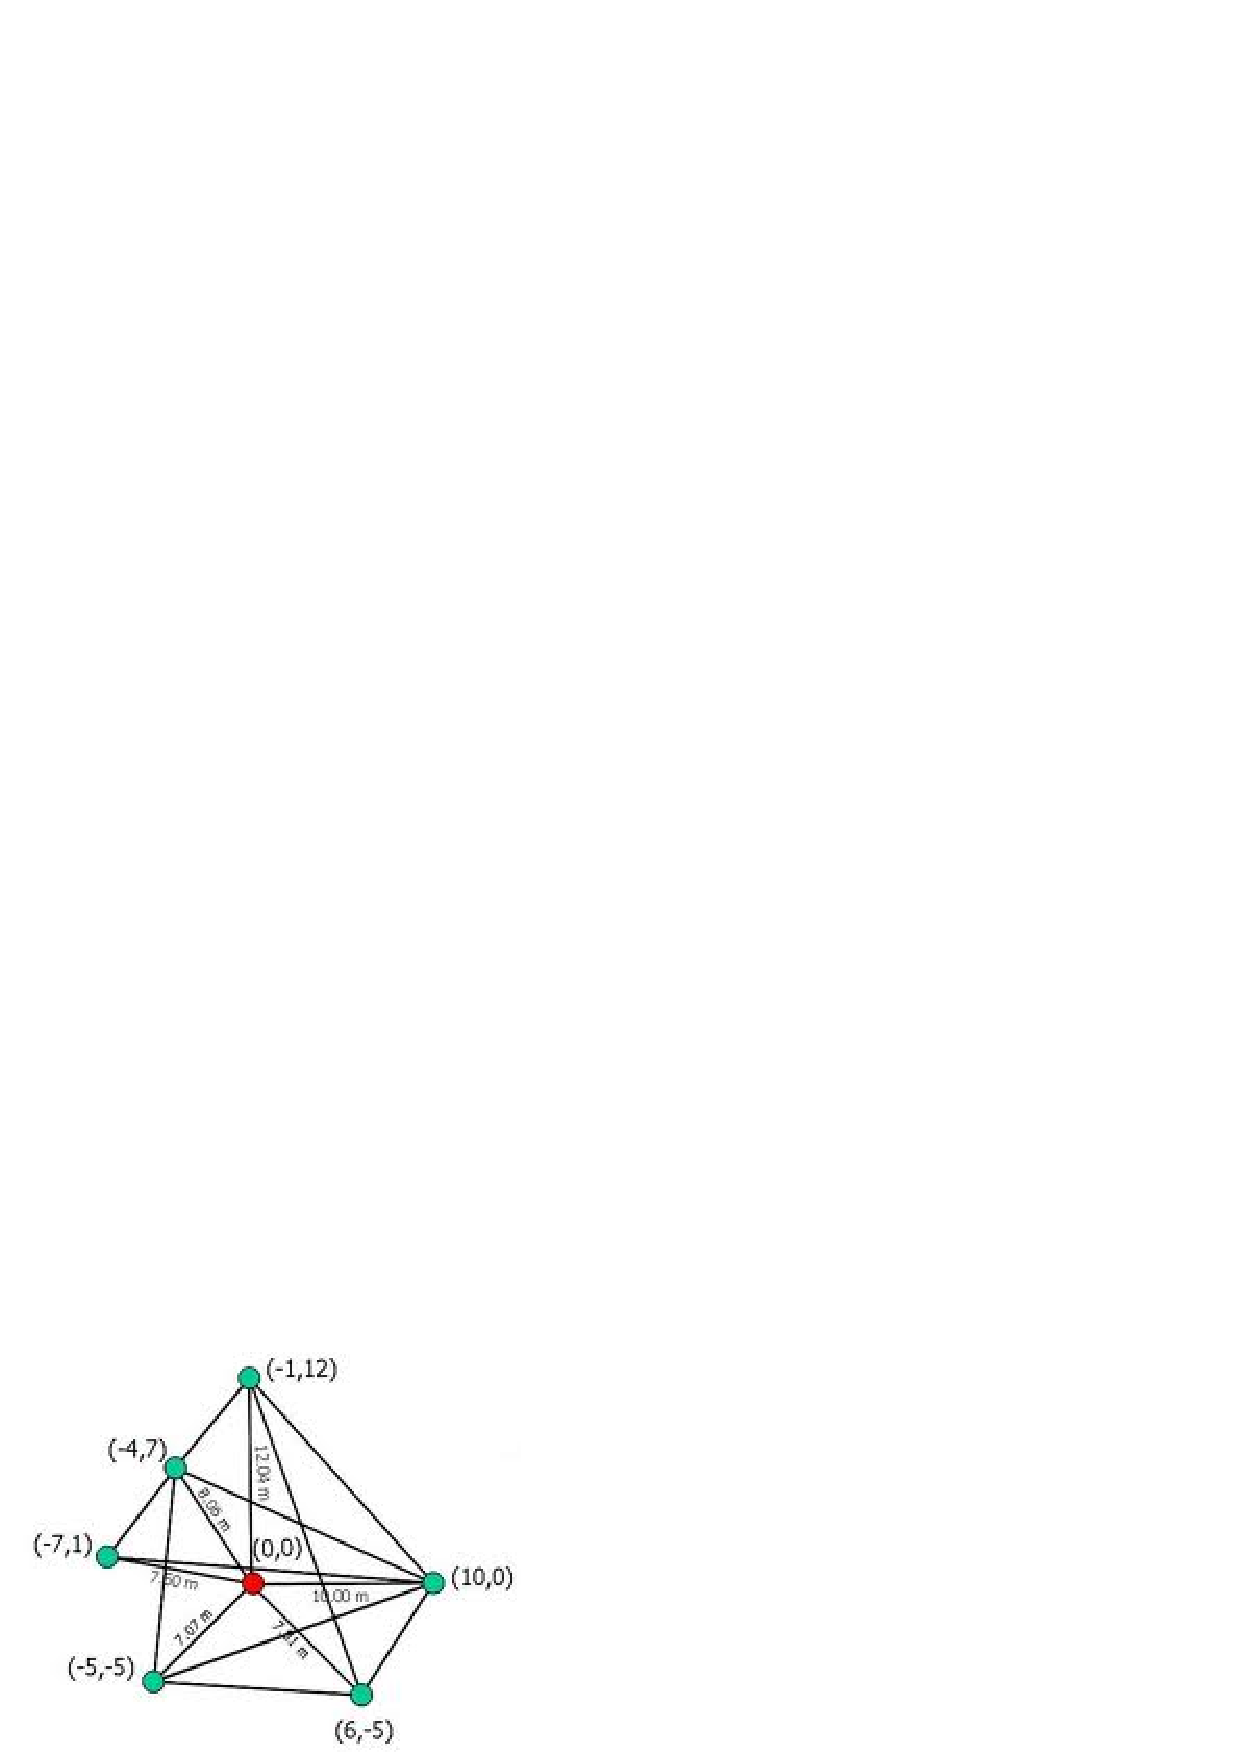
\includegraphics[width=5cm]{GraphRealization.jpg} }
  \subfigure{ 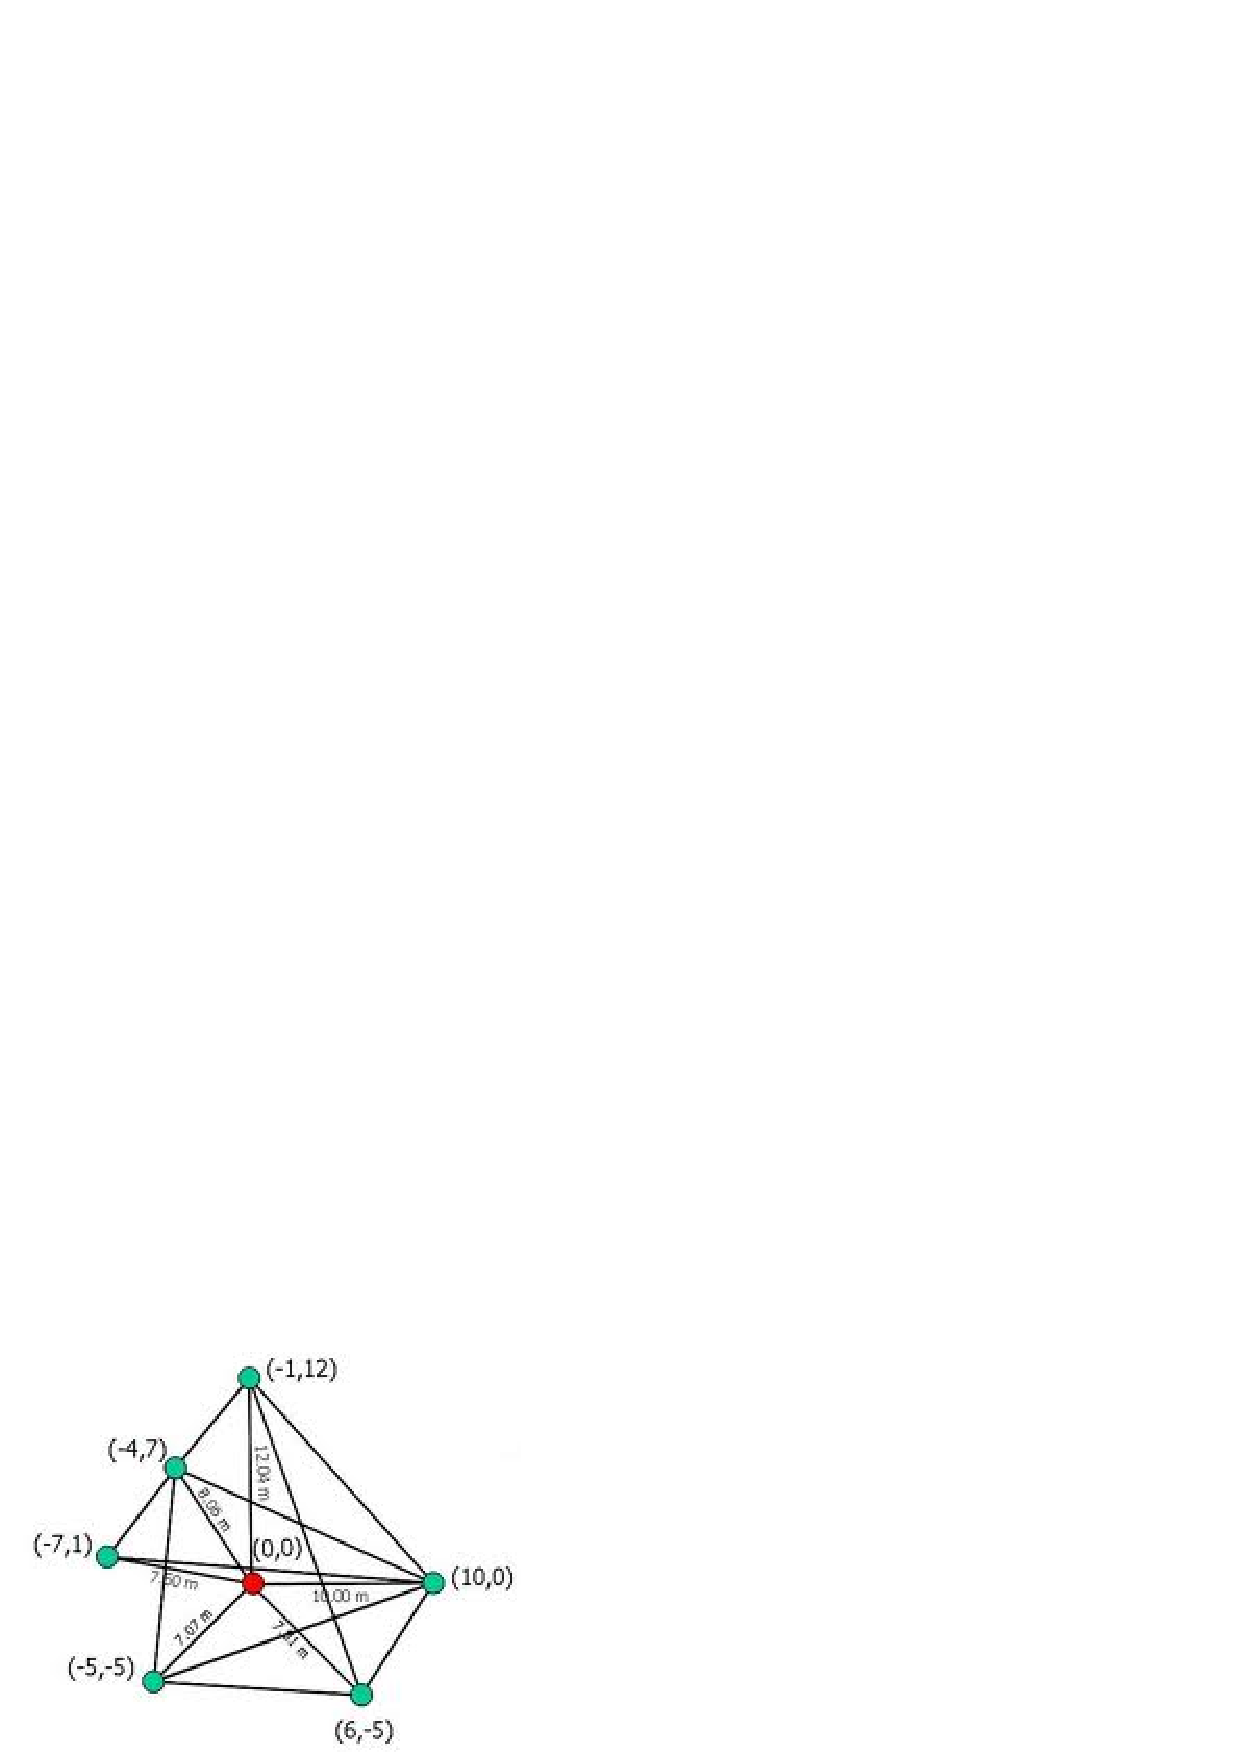
\includegraphics[width=5cm]{GraphRealization2.jpg} }
  \caption{Graph Realization in 2D}
\end{figure}
}

\frame{
\frametitle{Application \Rmnum{2}: Protein Structure Determination}
\begin{figure}[htp]
    \centering
    \subfigure{\includegraphics[width=5cm]{1PTQ2.jpg} }
    \subfigure{\includegraphics[width=5cm]{1HQQ2.jpg} }
    \caption{Two proteins: 1PTQ and 1HQQ, in different display ways}
\end{figure}
}

\frame{
\frametitle{Application \Rmnum{3}: Sensor Network Localization}
\begin{figure}[htp]
    \centering
    \subfigure{\includegraphics[width=4.5cm]{sensor2.jpg} }
    \subfigure{\includegraphics[width=4.5cm]{sensor1.jpg} }
    \caption{Illustration of wireless sensor networks}
\end{figure}
}

\section{Related works}
\frame{
\frametitle{Related works}
\begin{itemize}%[$\blacktriangleright$]
  \item Matrix Decomposition Method (Blumenthal 1953, Torgerson 1958)
  \item The Embedding Algorithm (Crippen, Havel 1988)
  \item Global Smoothing Algorithm (Mor\'{e}, Wu 1997)
  \item Geometric Buildup Method (Dong, Wu 2002)
  \item SDP Relaxation Method (Biswas et al., 2006)
  \item ...
\end{itemize}
}

\frame{
\frametitle{Matrix Decomposition Method}
{\red DG problem with full set of exact distances} \\
%\textrm{}\\
\small{
Given a full set of distances, $d_{i,j} = \| x_{i}-x_{j} \|, \quad i,j=1,2,\ldots,n.$ \\
\begin{itemize}%[$\blacktriangleright$]
  \item Set $x_{n} = (0,0,0\Tran)$, we have
      \begin{eqnarray}
      % \nonumber to remove numbering (before each equation)
        \nonumber d_{i,j}^{2} &=& \|x_{i}-x_{j}\|^{2} \\
        \nonumber             &=& \|x_{i}\|^{2}-2\Tran x_{i} x_{j}+\|x_{j}\|^{2} \\
                              &=& d_{i,n}^{2}-2\Tran x_{i} x_{j}+d_{j,n}^{2}, \qquad  i,j=1,2,\ldots,n-1 \label{eq1}
      \end{eqnarray} \\
      \vspace{0.3cm}
  \item Define $ X=(x_{1},x_{2},\ldots,x_{n}\Tran)$ and $D=\{(d_{i,n}^{2}-d_{i,j}^{2}+d_{j,n}^{2})/2: i,j=1,2,\ldots,n-1\}$,  (\ref{eq1}) $\Rightarrow {\red X\Tran X=D}$.\\
      \vspace{0.3cm}
  \item Let $D=U\Sigma\Tran U$, $V=U(:,1:3)$ and $\Lambda=\Sigma(1:3,1:3)$. Then $X = V\Lambda^{1/2}$ solves the problem. [{\blue Eckart and Young 1936}]
\end{itemize} }
}

\frame{
\frametitle{Unconstrained optimization: Error functions}
\begin{itemize}
  \item stress function
        \begin{equation*}
          Stress(x_{1},x_{2},\ldots,x_{n}) = \sum_{(i,j)\in S} (\|x_{i}-x_{j}\|-d_{i,j})^{2},
        \end{equation*}
  \item smoothed stress function
  \begin{equation*}
          SStress(x_{1},x_{2},\ldots,x_{n}) = \sum_{(i,j)\in S} (\|x_{i}-x_{j}\|^{{\red 2}}-d_{i,j}^{{\red 2}})^{2},
        \end{equation*}
  \item generalized stress function
        \footnotesize{
        \begin{equation*}
          GStress(x_{1},x_{2},\ldots,x_{n}) = \sum_{(i,j)\in S} \min\nolimits^{2} \{\frac{\|x_{i}-x_{j}\|^{2}-l_{i,j}^2}{l_{i,j}^{2}},0\} + \max\nolimits^{2} \{\frac{\|x_{i}-x_{j}\|^{2}-u_{i,j}^2}{u_{i,j}^{2}},0\}.
        \end{equation*} }
\end{itemize}
}

\frame{
\frametitle{Goal and Difficulties}
\begin{itemize}
  \item Goal: minimize the chosen error function to the {\red global} minimizer---{\red zero}
      \vspace{0.3cm}
  \item Difficulties: NP-hard in general
  \begin{enumerate}[--]
    \item too many local minimizers
    \item possibly nonsmooth
    \item large-scale problems
  \end{enumerate}
\end{itemize}
}

\section{Our proposed error function and algorithm}
\frame{
\frametitle{Our proposed error function}
\begin{minipage}{0.45\textwidth}
Define h: $\mathbb{R}_{++}\rightarrow \mathbb{R}$ as below,
\begin{displaymath}
  h(x) = \left\{ \begin{array}{ll}
                  \frac{1}{2}(x-1)^{2}, & x\geq 1, \\
                  x-(1+ln(x)),          & x<1.
                \end{array}   \right.
\end{displaymath}
\end{minipage}
\begin{minipage}{0.45\textwidth}
\begin{figure}
  \centering
  \includegraphics[width=\textwidth]{huke.jpg}
\end{figure}
\end{minipage}

\textrm{}\\
\begin{Thm}
h(x) is twice continuously differentiable in $(0, +\infty)$, and it achieves its minimum 0 at 1.
\end{Thm}
}

\frame{
\frametitle{Modeling and Solution idea}
Using our error function, the distance geometry problem can be formulated as
{\red
\begin{equation}
  \min \quad f(x_{1},x_{2},\ldots,x_{n})=\sum_{(i,j)\in S} h(\frac{\|x_{i}-x_{j}\|}{d_{i,j}}).
\end{equation} }
\vspace{0.3cm}
\begin{itemize}
  \item Observation:
  \begin{enumerate}[--]
    \item huge items in the objective function
    \item variables are mixed together $\Rightarrow$ not easy to calculate Hessian matrix
  \end{enumerate}
  \item Solution idea:
  \begin{enumerate}[--]
    \item use first-order algorithm --- "alternative direction method" to solve it\\
    $\Rightarrow$ fixed the others, adjust $x_{i}(i=1,\ldots,n)$ in turn.
  \end{enumerate}
\end{itemize}
}


\frame{
\frametitle{Trust region subproblem}
Let $\overline{f}(x)=\sum_{j\in N(i)} h(\frac{\|x-x_{j}\|}{d_{i,j}})$, where $N(i)$ is the neighbourhood of point $i$, then the "trust region subproblem" at each iteration is as following,
\begin{equation}\label{tr}
  \begin{array}{ccl}
  \min\limits_{s} & \Tran{s}\nabla\overline{f}(x_{i}) + \frac{1}{2}\Tran{s}\nabla^{2}\overline{f}(x_{i})s & \triangleq q(x) \\
  \st      & \|s\| \leq \Delta. & \\
  \end{array}
\end{equation}
\begin{figure}
  \centering
  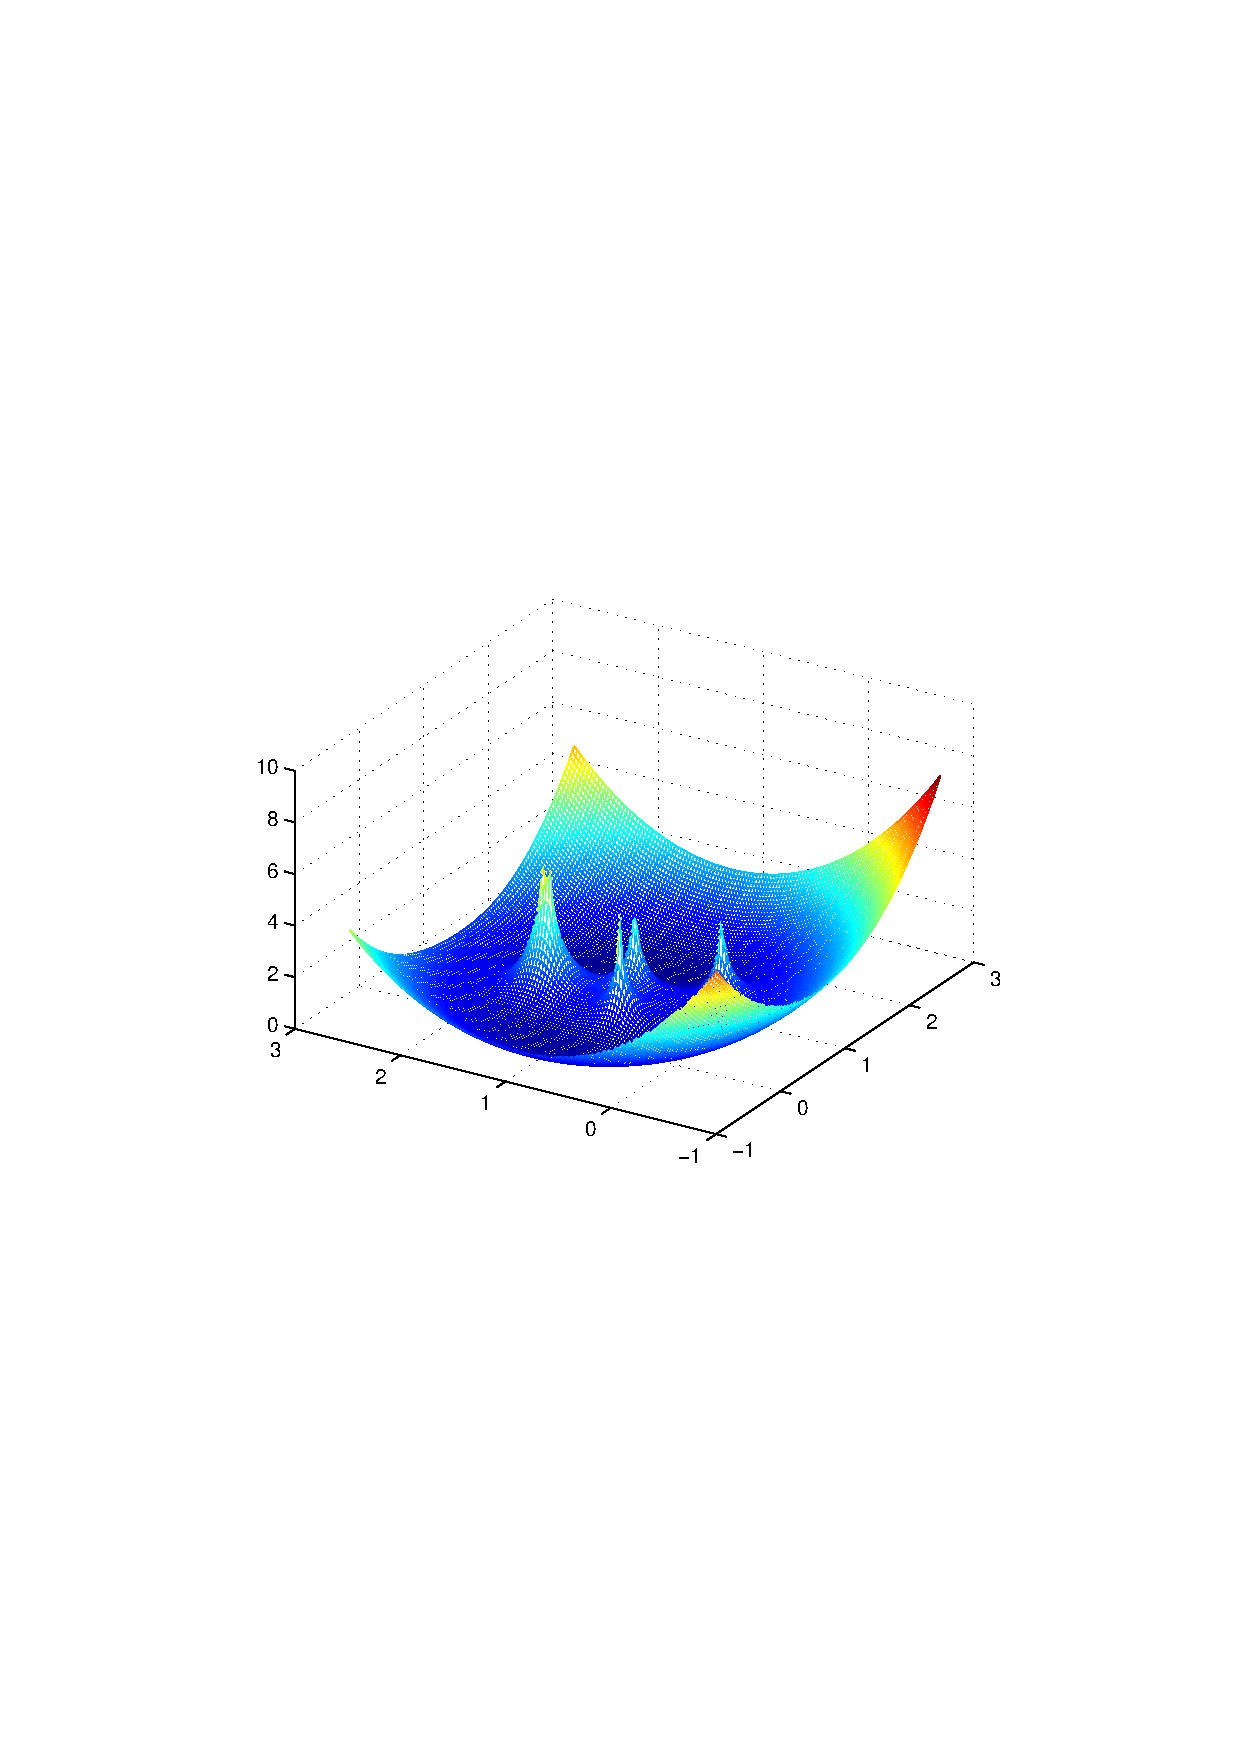
\includegraphics[width=0.5\textwidth]{energy.jpg}\\
  %\caption{Illustration of $\overline{f}(x)$}
\end{figure}
}

\frame{
\frametitle{Trust region subproblem (Cont'd)}
\footnotesize{
\begin{Thm}
Define $\overline{h}: \Real^{d}\rightarrow \Real, \overline{h}(x)=h(\frac{\|x-a\|}{d})$, where $a\in \Real^{d}$ and $d\in \Real$ are constants, then
\begin{itemize}
  \item $$ \nabla \overline{h}(y)=\frac{y}{d\|y\|}-\frac{y}{\|y\|^{2}},$$
  and
$$ \nabla^{2} \overline{h}(y)=-\frac{y\Tran{y}}{d\|y\|^{3}} + \frac{2y\Tran{y}}{\|y\|^{4}} + (\frac{1}{d\|y\|}-\frac{1}{\|y\|^{2}})I$$
$$\qquad \quad=(\frac{1}{d\|y\|}-\frac{1}{\|y\|^{2}})(I-\frac{y\Tran{y}}{\|y\|^{2}}) + \frac{y\Tran{y}}{\|y\|^{4}},$$
where
$$y=x-a \textrm{ and I is the identity matrix}.$$
  \item if $\|y\| \geq d, \nabla^{2} \overline{h} (y)$ is positive definite, otherwise it can be negative definite.
\end{itemize}
\end{Thm} }
}

\frame{
\frametitle{Stopping criteria}
\begin{enumerate}
  \item the objective function or the improvement is small enough, i.e.
  $$f_{k}< tol~~~or~~~|f_{k}-f_{k-1}|< tol$$
  \item the norm of the gradient is small enough, i.e.
  $$\|\nabla f(x)\|< MinNorm$$
  where $tol,~MinNorm$ are some given small numbers, for instance, $10^{-5}$.
  \item the outer iteration achieves its maximum permitted number, i.e. $k<MaxItr$
\end{enumerate}
\vspace{0.5cm}
\begin{enumerate}[{\color{black} $\spadesuit$ }]
  \item One of the above three criteria is satisfied, the algorithm will stop.
\end{enumerate}
}

\frame{
\frametitle{Algorithm framework \Rmnum{1}}
\begin{algorithm}[H]
\SetKwInOut{Init}{Initialization}
\vspace{0.3cm}
\Init{Give initial points and set some parameters}
\While{stopping criteria not satisfied}{
\For{i=1:n}{ Solve trust region subproblem (\ref{tr}) to obtain $s_{i}$, let
$$r_{i} = \frac{\overline{f}(x_{i})-\overline{f}(x_{i}+s_{i})}{q(x_{i})-q(x_{i}+s_{i})}$$
According to $r_{i}$ to determine to accept $s_{i}$ or not, and adjust $\Delta_{i}$\;
}
}
\caption{Trust Region Error Minimization Method}
\label{algtr}
\end{algorithm}
}

\frame{
\frametitle{Nonmonotone Newton step}
\begin{itemize}
  \item Let $\overline{f}(x)$ be defined as before, then "Newton step" can be given as below,
      $$d_{i}^{N} = -(\nabla^{2}\overline{f}(x_{i}))^{-1}\nabla\overline{f}(x_{i})$$
      Let search direction be
      \begin{equation}\label{Ndirection}
      d_{i} = \left\{
      \begin{array}{ll}
      d_{i}^{N} & if~\nabla^{2}\overline{f}(x_{i})~is~positive~definite,\\ -\nabla\overline{f}(x_{i}) & otherwise,
      \end{array} \right.
      \end{equation}
      which is a descent direction.
  \item Search for stepsize $\alpha_{i}$ by backtracking (start at 1), such that
      \begin{equation}\label{Nstepsize}
      f(x_{i}+\alpha_{i}d_{i},x_{-i})< MaxF + \frac{1}{2}\alpha_{i}\Tran{d_{i}}\nabla\overline{f}(x_{i})%\max_{k=1:M} {fval(i-k)}
      \end{equation}
      where $MaxF$ is the maximum objective function value of lastest M step.
\end{itemize}
}

\frame{
\frametitle{Algorithm framework \Rmnum{2}}
\begin{algorithm}[H]
\SetKwInOut{Init}{Initialization}
\vspace{0.3cm}
\Init{Give initial points and set some parameters}
\While{stopping criteria not satisfied}{
\For{i=1:n}{
Calculate search direction $d_{i}$ by (\ref{Ndirection})\;
Calculate stepsize $\alpha_{i}$ by (\ref{Nstepsize})\;
Set $x_{i}\leftarrow x_{i}+\alpha_{i}d_{i}$
}
}
\caption{Nonmonotone Newton Error Minimization Method}
\label{algNewton}
\end{algorithm}
}

\frame{
\frametitle{Algorithm framework \Rmnum{3}}
\begin{algorithm}[H]
\vspace{0.4cm}
\begin{enumerate}
  \item Apply \textbf{Algorithm \ref{algtr}} for K iterations,
  \item Apply \textbf{Algorithm \ref{algNewton}} then.
\end{enumerate}
\caption{Trust Region-Newton Error Minimization Method}
\end{algorithm}
}

\section{Numerical experiments}
%\frame{
%\frametitle{Problem and parameters}
%\begin{itemize}
%  \item Download structure data from Protein Data Bank(PDB), obtain the original coordinates X.
%  \item Use \emph{{\blue disk graph model}} to construct distance matrix, usually set cutoff as 5{\AA} or 6{\AA}.
%  \item Solve the problem with our algorithm to get Computed coordinates Y, then compare it with X, using the criteria defined as below,
%        $$ RMSD(X,Y) = \min_{Q,T}\|X-YQ-T\|_{F}/\sqrt{n} $$
%\end{itemize}
%}

\frame{
\frametitle{Experiments construction}
\begin{itemize}
  \item Uniformly sample nodes in square [0,1]x[0,1];
  \item Generate distance matrix by \emph{disk graph model}, usually set cutoff=0.2, thus about 10\% distance are available.
  \item Generate initial points with 20\% perturbation, more specifically,
      $$X0 = X + 0.2*(rand(n,2)-0.5),$$
  \item Use function value and cost time as the compare criteria.
\end{itemize}
}

\frame{
\frametitle{Monotone VS Nonmonotone stepsize}
\centering
\begin{tabular}{|r|c|c|c||r|c|c|c|}
  \hline
  \multicolumn{8}{|c|}{$cotoff=0.2, exact~distance, perturbation=20\%, MaxItr=100$} \\
  \hline
  \multicolumn{4}{|c||}{$n=100, tol=10^{-3}$} & \multicolumn{4}{c|}{$n=200, tol=10^{-3}$} \\
  \hline
  M & Itr & fval & t(s) & M & Itr & fval & t(s)\\
  \hline
    1 & 17 & 0.080 & 3.37 &   1 & 100 & 5.206 & 40.40 \\
    5 & 35 & 0.012 & 3.98 &   5 & 100 & 4.170 & 34.17 \\
   20 & 32 & 0.014 & 3.86 &  20 & 100 & 1.893 & 34.36 \\
   50 & 35 & 0.012 & 4.00 &  50 & 100 & 0.263 & 32.44 \\
  100 & 30 & 0.013 & 3.76 & 100 & 100 & {\blue 0.112} & 31.63\\
  \hline
    1 & 36 & 0.474 & 5.30 &   1 &  84 & 0.430 & 31.03 \\
    5 & 31 & 0.462 & 4.46 &   5 &  65 & 0.417 & 24.25 \\
   20 & 30 & 0.459 & 4.42 &  20 &  63 & 0.417 & 23.88 \\
   50 & 28 & 0.456 & 4.33 &  50 &  63 & 0.416 & 23.82 \\
  100 & 28 & 0.456 & 4.33 & 100 &  63 & 0.415 & 23.81 \\
  \hline
\end{tabular} \\
}

\frame{
\frametitle{Monotone VS Nonmonotone stepsize}
\centering
\begin{tabular}{|r|c|c|c||r|c|c|c|}
  \hline
  \multicolumn{8}{|c|}{$cotoff=0.2, exact~distance, perturbation=20\%, MaxItr=100$} \\
  \hline
  \multicolumn{4}{|c||}{$n=500, tol=10^{-2}$} & \multicolumn{4}{c|}{$n=1000, tol=10^{-1}$} \\
  \hline
  M & Itr & fval & t(s) & M & Itr & fval & t(s)\\
  \hline
    1 & 100 & 27.840 & 193.64 &   1 & 100 & 476.719 & 949.58 \\
    5 & 100 & {\blue18.176} & 158.75 &   5 &  57 & 495.770 & 550.68 \\
   20 & 100 & 27.614 & 162.99 &  20 &  65 & 288.151 & 574.78 \\
   50 & 100 & 22.696 & 158.43 &  50 &  90 & {\blue 112.026} & 667.39 \\
  100 & 100 & 29.526 & 157.47 & 100 &  75 & 127.622 & 5146.84 \\
  \hline
    1 & 100 & 56.317 & 209.39 &   1 &  57 & 395.741 & 722.18 \\
    5 & 100 & 53.942 & 177.58 &   5 &  48 & 316.193 & 606.12 \\
   20 & 100 & 25.786 & 172.77 &  20 &  41 & 203.620 & 524.87 \\
   50 & 100 & 26.246 & 168.34 &  50 &  41 & {\blue 57.026} & 495.40 \\
  100 & 100 & {\blue 23.701} & 169.85 & 100 &  41 &  97.319 & 520.48 \\
  \hline
\end{tabular} \\
}

\frame{
\frametitle{Monotone Newton}
\begin{figure}
  \centering
  \includegraphics[width=0.9\textwidth]{ff2.jpg}\\
\end{figure}
}

\frame{
\frametitle{Trust region VS Newton}
\centering
\begin{tabular}{|r|c|c|c||r|c|c|c|}
  \hline
  \multicolumn{8}{|c|}{$cotoff=0.2, exact~distance, perturbation=20\%, MaxItr=150$} \\
  \hline
  \multicolumn{4}{|c||}{$n=200, tol=10^{-3}$} & \multicolumn{4}{c|}{$n=500, tol=10^{-2}$} \\
  \hline
  Alg & Itr & fval & t(s) & Algo & Itr & fval & t(s)\\
  \hline
  Alg1 & 150 & 12.234 & 40.35 & Alg1 & 150 & 167.611 & 230.60 \\
  Alg2 & 150 &  1.234 & 38.17 & Alg2 & 150 & 221.197 & 312.59 \\
  Alg3 & 129 &  0.531 & 26.97 & Alg3 & 150 &  11.380 & 197.97 \\
  \hline
  Alg1 & 150 & 11.500 & 39.91 & Alg1 & 150 & 302.333 & 222.11 \\
  Alg2 & 150 &  5.305 & 37.93 & Alg2 & 150 & 119.509 & 273.53 \\
  Alg3 & 150 &  0.269 & 30.68 & Alg3 & 150 &  24.185 & 186.34 \\
  \hline
  Alg1 & 150 & 27.146 & 37.68 & Alg1 & 150 & 273.636 & 226.34 \\
  Alg2 & 150 &  9.764 & 36.75 & Alg2 &  93 & 188.148 & 185.29 \\
  Alg3 & 150 &  0.365 & 30.10 & Alg3 & 150 &  49.415 & 206.23 \\
  \hline
\end{tabular} \\
}

\frame{
\frametitle{Trust region VS Newton}
\begin{figure}
  \centering
  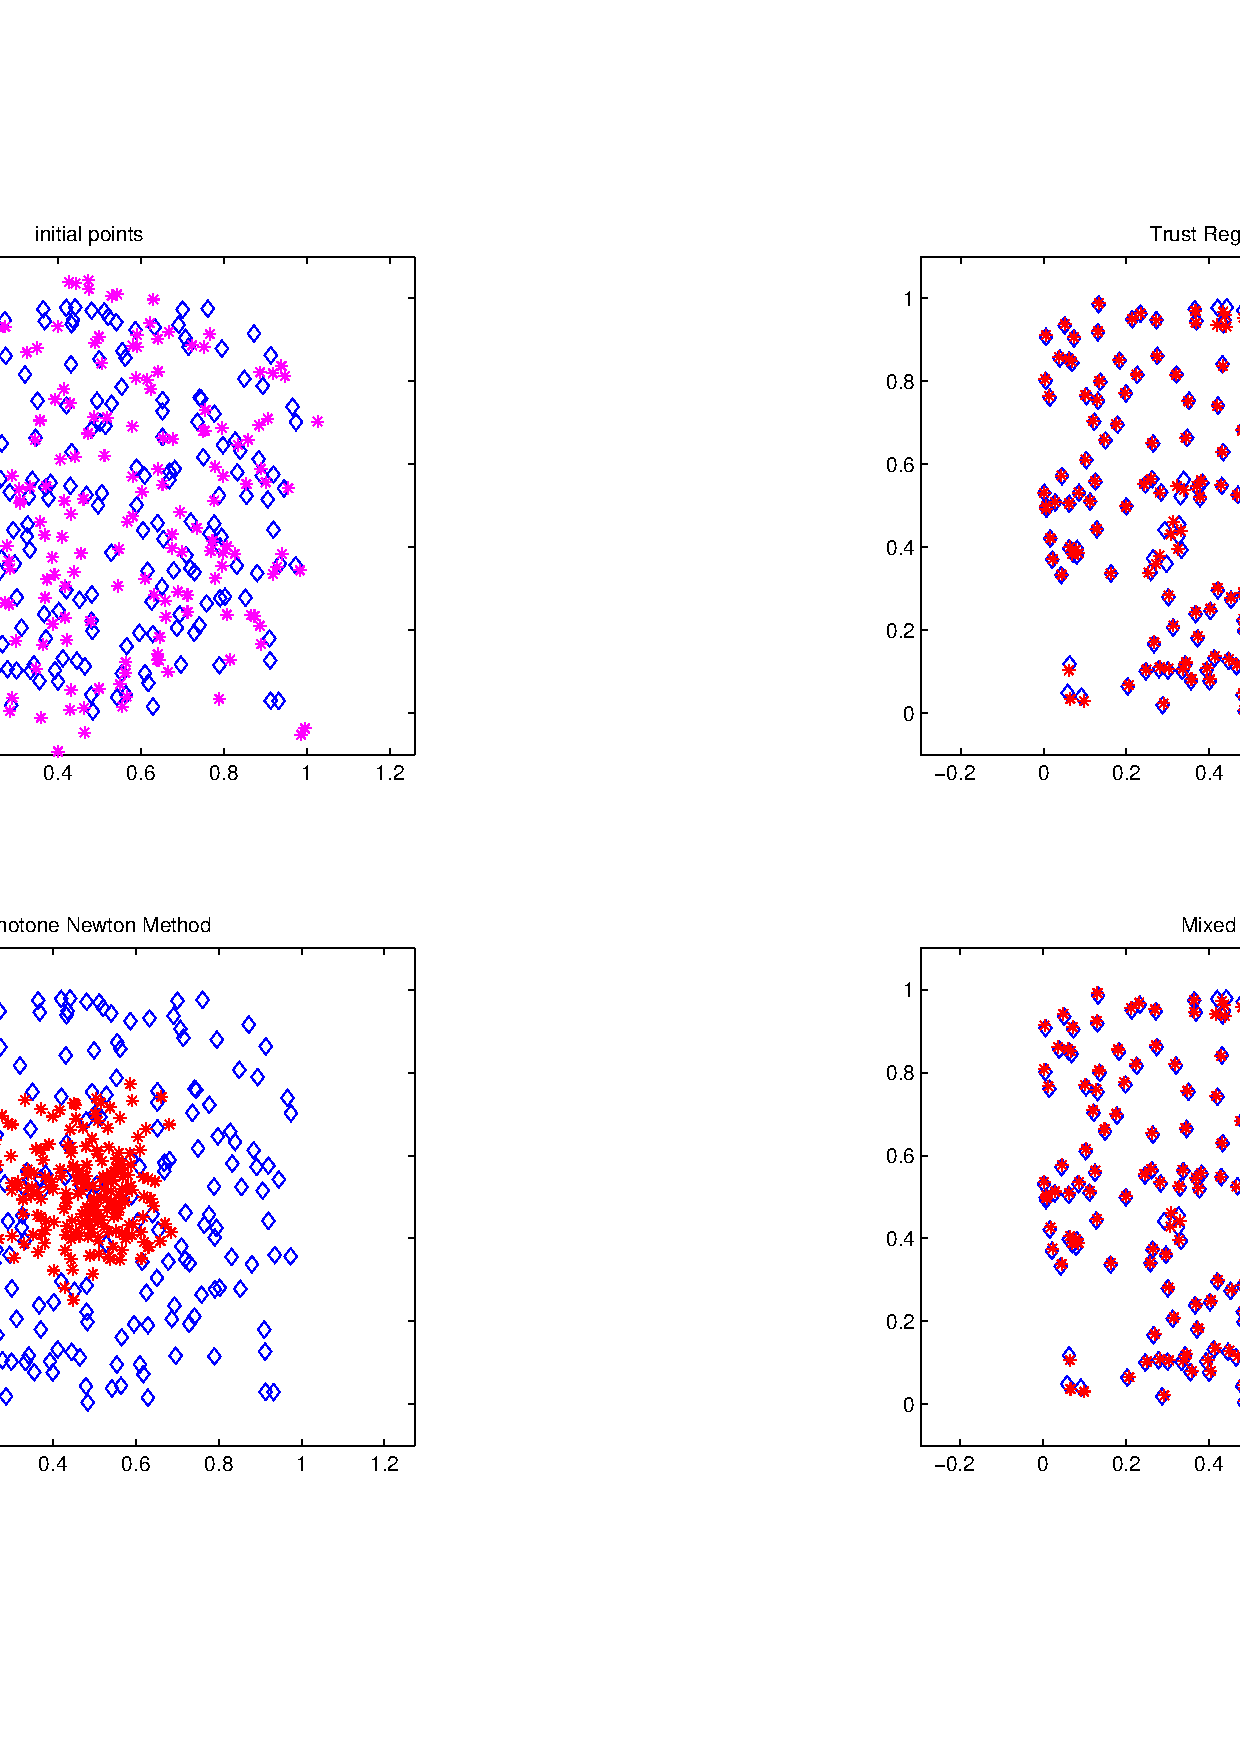
\includegraphics[width=0.9\textwidth]{TrNewton.jpg}\\
\end{figure}
}

\frame{
\frametitle{Trust region VS Newton}
\begin{figure}
  \centering
  \includegraphics[width=0.7\textwidth]{TrNewtonFval.jpg}\\
  \caption{An typical example: 200 nodes, exact distance, 20\% perturbation}
\end{figure}
}

\frame{
\frametitle{Trust region VS Newton}
\begin{figure}
  \centering
  \includegraphics[width=0.9\textwidth]{TrNewton500.jpg}\\
\end{figure}
}

\frame{
\frametitle{Trust region VS Newton}
\begin{figure}
  \centering
  \includegraphics[width=0.7\textwidth]{TrNewtonFval500.jpg}\\
  \caption{An typical example: 500 nodes, exact distance, 20\% perturbation}
\end{figure}
}

\frame{
\frametitle{exact VS noise distances}
\centering
\begin{tabular}{|r|c|c|c||r|c|c|c|}
  \hline
  \multicolumn{8}{|c|}{$cotoff=0.2, perturbation=20\%, MaxItr=150, tol=10^{-3}$} \\
  \hline
  \multicolumn{4}{|c||}{$n=200, noise=1\%$} & \multicolumn{4}{c|}{$n=200, noise=5\%$} \\
  \hline
  dist & Itr & fval & t(s) & dist & Itr & fval & t(s)\\
  \hline
  exact & 150 &  1.548 & 30.52 & exact & 150 &  0.111 & 31.22 \\
  noise & 150 &  0.304 & 30.64 & noise & 150 &  1.665 & 30.93 \\
  \hline
  exact & 137 &  0.137 & 29.65 & exact & 148 &  1.060 & 29.94 \\
  noise & 136 &  0.677 & 30.55 & noise & 150 &  1.167 & 30.32 \\
  \hline
  \multicolumn{4}{|c||}{$n=200, noise=10\%$} & \multicolumn{4}{c|}{$n=200, noise=20\%$} \\
  \hline
  exact & 143 &  0.037 & 30.05 & exact & 143 &  0.420 & 28.71 \\
  noise & 150 &  0.734 & 31.07 & noise & 150 &  5.265 & 30.06 \\
  \hline
  exact & 150 &  0.516 & 29.57 & exact & 109 &  0.057 & 22.83 \\
  noise & 150 &  2.134 & 29.68 & noise &  77 &  5.068 & 18.23 \\
  \hline
\end{tabular} \\ }

\frame{
\frametitle{Trust region VS Newton}
\begin{figure}
  \centering
  \includegraphics[width=0.9\textwidth]{noise1.jpg}\\
  %\caption{An typical example of graph with 200 nodes, 1\% noise distance}
\end{figure}
}

\frame{
\frametitle{Trust region VS Newton}
\begin{figure}
  \centering
  \includegraphics[width=0.9\textwidth]{noise5.jpg}\\
  %\caption{An typical example of graph with 200 nodes, 5\% noise distance}
\end{figure}
}

\frame{
\frametitle{Trust region VS Newton}
\begin{figure}
  \centering
  \includegraphics[width=0.9\textwidth]{noise10.jpg}\\
  %\caption{An typical example of graph with 200 nodes, 10\% noise distance}
\end{figure}
}

\frame{
\frametitle{Trust region VS Newton}
\begin{figure}
  \centering
  \includegraphics[width=0.9\textwidth]{noise20.jpg}\\
  %\caption{An typical example of graph with 200 nodes, 20\% noise distance}
\end{figure}
}

\section{Conclusions and Future work}
\frame{
\frametitle{Conclusions and Future work}
\begin{itemize}%[$\blacktriangleright$]
  \item What we have done:
        \begin{enumerate}[--]
          \item proposed a novel error function
          \item based on the proposed function, designed an efficient algorithm to solve the distance geometry problem
          \item finished some preliminary numerical experiments, which seems promising, especially in the noise case
        \end{enumerate}
  \item Future work:
        \begin{enumerate}[--]
          \item theoretical convergence analysis of the algorithm
          \item generalize the error function to handle the "bound" case
          \item compare the algorithm with the existing ones
        \end{enumerate}
\end{itemize}
}

\frame{
\frametitle{Q \& A}
\begin{center}
  \Large {\blue \textsc{Thank you for your attention!} }
\end{center}
}

\end{CJK*}
\end{document}
